\chapter{Anhang}
\label{ch:anhang}

Dieses Kapitel enthält ergänzende Materialien, die für das Verständnis der Arbeit nicht
zwingend erforderlich, aber für die Nachvollziehbarkeit einzelner Ergebnisse hilfreich sind.

% ─────────────────────────────────────────────────────────────

\section{Vollständiges Entity-Relationship-Diagramm}
\label{sec:anhang_erd}

Das folgende Diagramm zeigt das vollständige Entity-Relationship-Diagramm der
EffSync-Datenbank. Es umfasst alle Tabellen und Beziehungen, von denen in
Kapitel~\ref{ch:systemarchitektur} und \ref{ch:implementierung_kernfunktionen}
jeweils nur Ausschnitte dargestellt wurden.

\begin{figure}[p]
    \centering
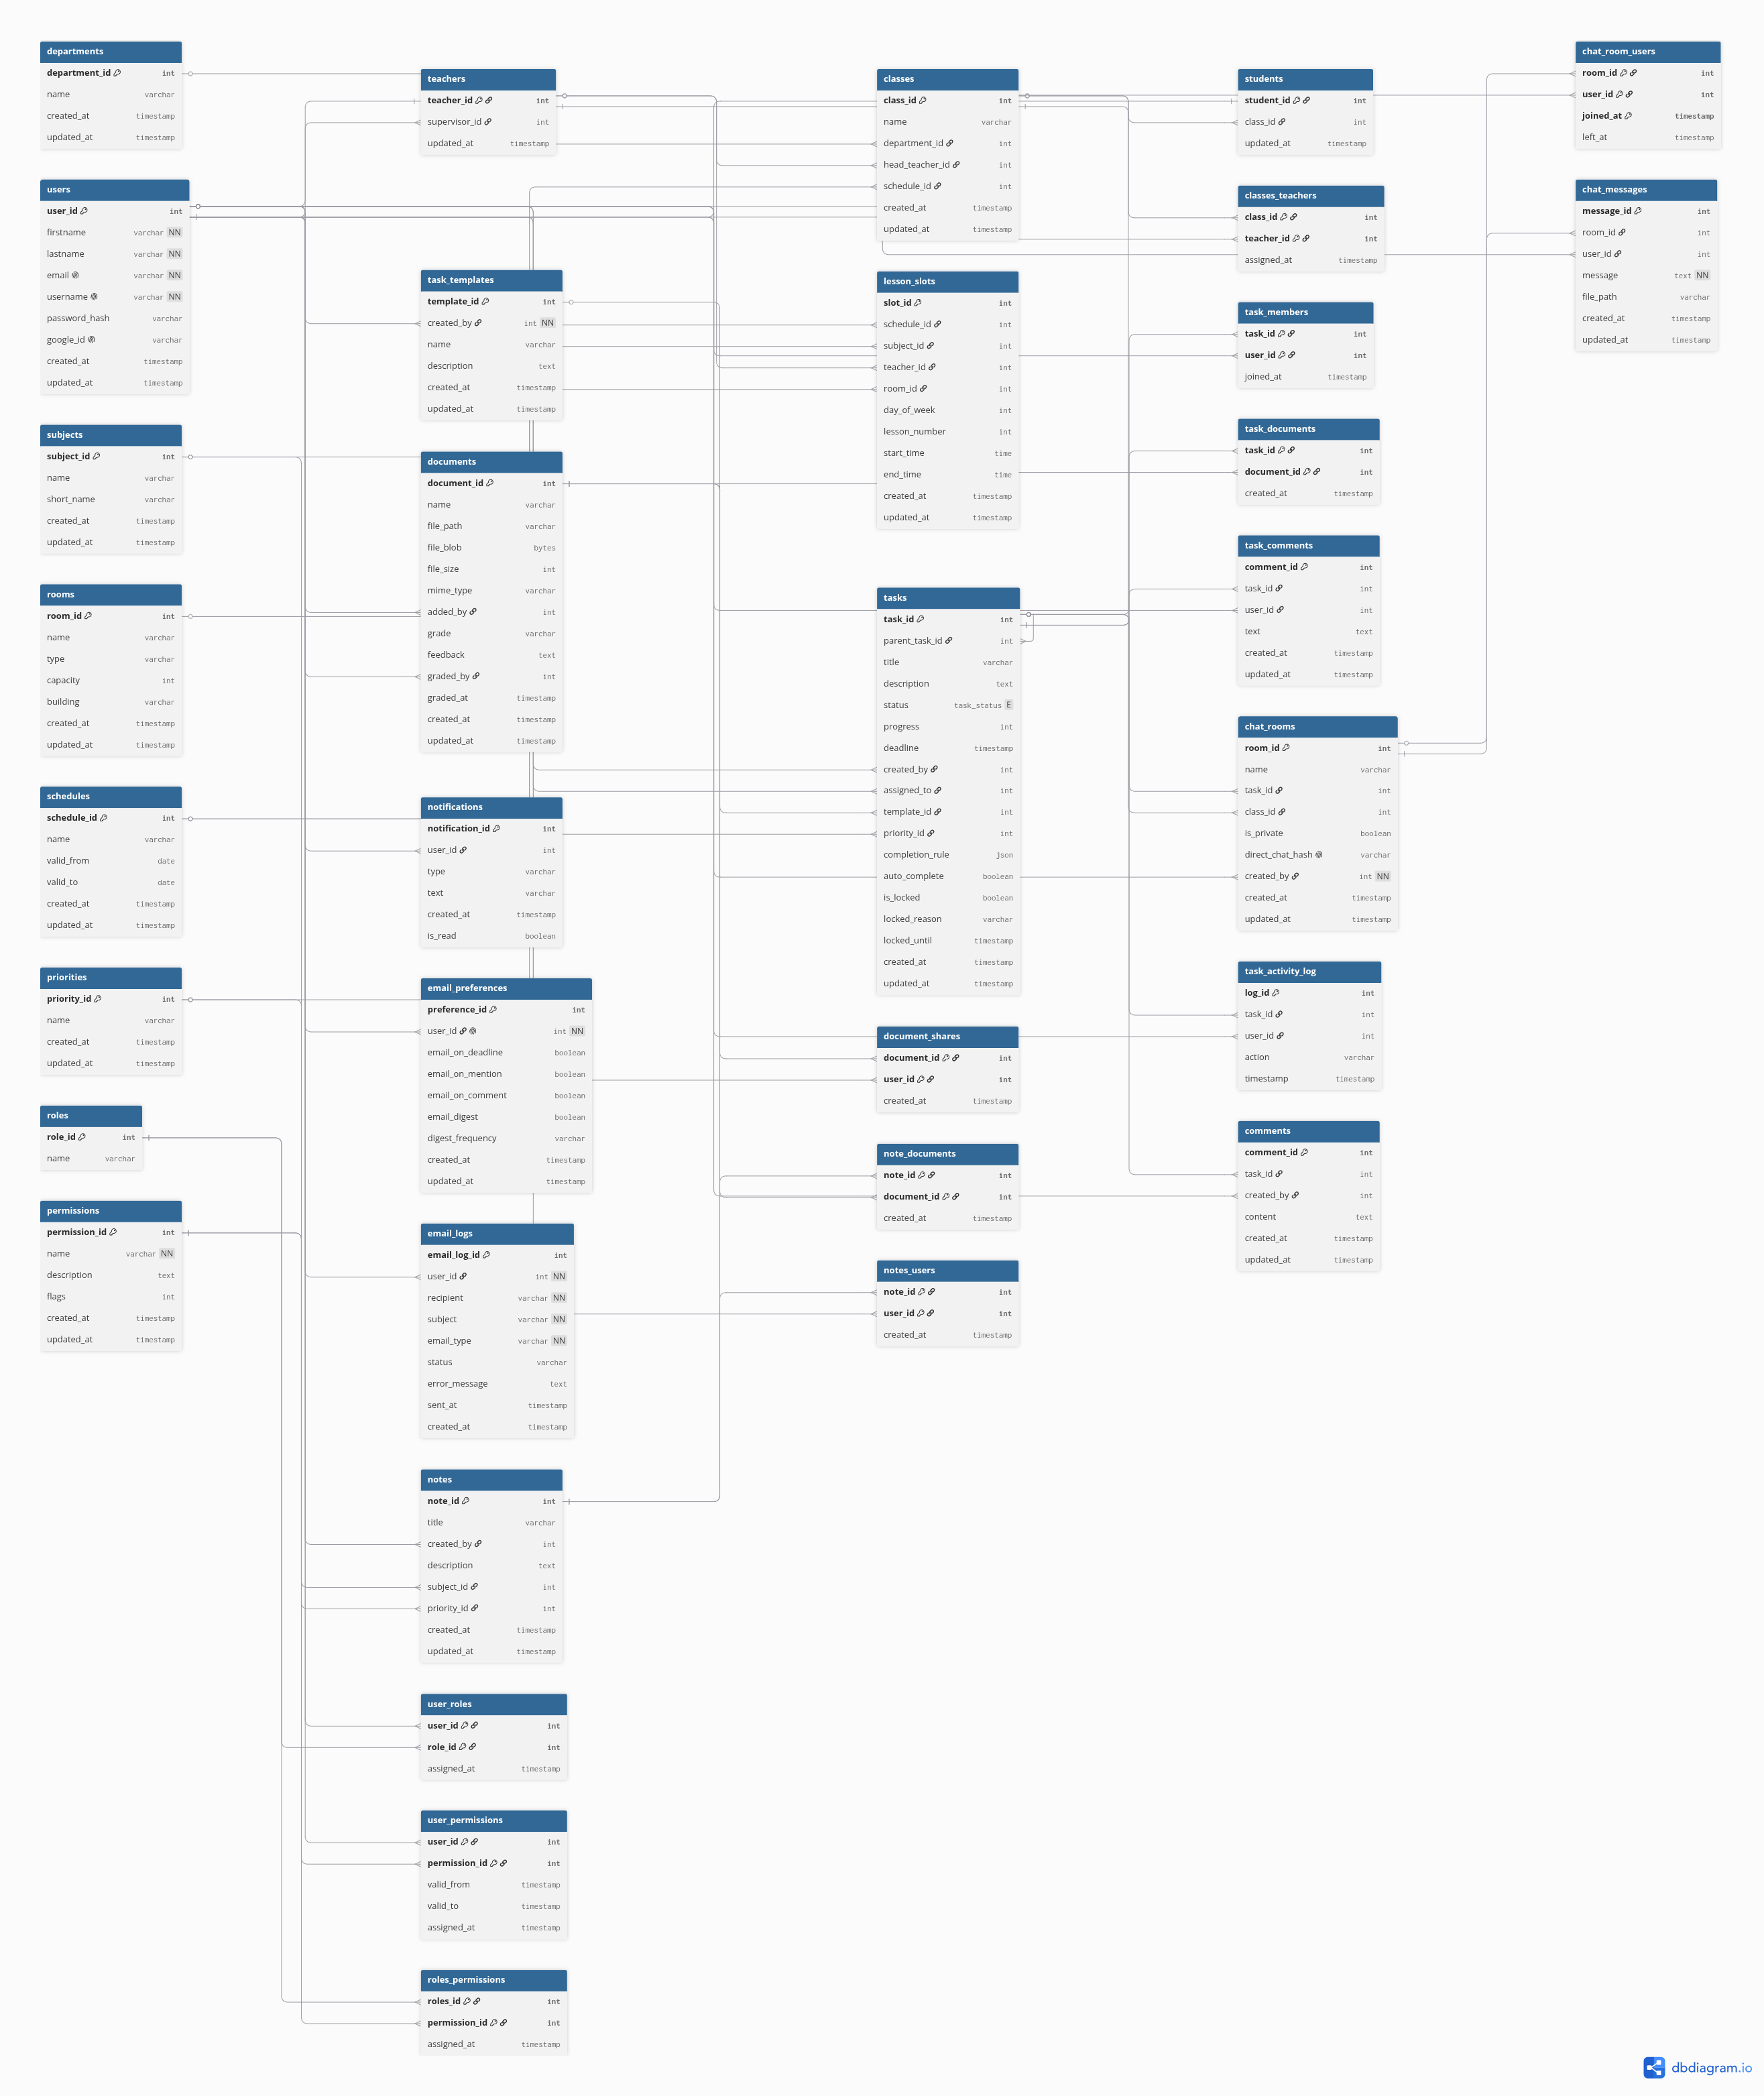
\includegraphics[width=\textwidth, height=\textheight, keepaspectratio]{content/bilder/Untitled.png}
    \caption{Vollständiges Entity-Relationship-Diagramm von EffSync}
    \label{fig:erd_vollstaendig}
\end{figure}

% ─────────────────────────────────────────────────────────────
\clearpage
\section{Fragebogen und Rohdaten des Usability-Tests}
\label{sec:anhang_usability}

Dieser Abschnitt enthält den vollständigen Aufgabenkatalog sowie die erhobenen
Rohdaten (Bearbeitungszeiten, Beobachtungsnotizen) des in
Abschnitt~\ref{sec:usability_test} beschriebenen Usability-Tests.


\subsection*{Effsync Usability-Test v2 (30 Minuten)}

\noindent
\textbf{Repository:} \url{https://github.com/kiDra94/diplom-arbeit} \\
\textbf{Datum:} \underline{\hspace{4cm}} \quad
\textbf{Testleitung:} \underline{\hspace{4cm}} \quad
\textbf{Test-ID:} \underline{\hspace{3cm}} \\
\textbf{Teilnehmer-Rolle:} $\square$ Schüler \quad $\square$ Lehrer \quad $\square$ Admin \\
\textbf{Browser A:} \underline{\hspace{3cm}} \quad
\textbf{Browser B:} \underline{\hspace{3cm}}

% ─────────────────────────────────────────────────────────────
\subsection*{1) Ablauf (für Testleitung)}

\begin{itemize}
    \item Intro: 2 Min
    \item Warm-up: 3 Min
    \item Szenario 1: 6 Min
    \item Szenario 2: 6 Min
    \item Szenario 3: 6 Min
    \item Cross-Browser-Chat: 5 Min
    \item Abschlussfragen: 2 Min
\end{itemize}

\noindent\textbf{Regel:} Nicht helfen, außer wenn Teilnehmer komplett feststeckt (nach ca. 90 Sek).

% ─────────────────────────────────────────────────────────────
\subsection*{2) Aufgabenblatt (Teilnehmer + Beobachtung)}

\subsubsection*{Aufgabe 1 – Orientierung unter Zeitdruck (6 Min)}

\noindent\textbf{Ziel (rollenabhängig):}
\begin{itemize}
    \item Schüler: letzte Aufgabe + Abgabedatum finden
    \item Lehrer: Stelle finden, um neue Aufgabe zu veröffentlichen
    \item Admin: Stelle finden, um Rollen/Rechte zu ändern
\end{itemize}

\noindent\textbf{Messung:} \\
Startzeit: \underline{\hspace{2cm}} \quad
Endzeit: \underline{\hspace{2cm}} \quad
Dauer: \underline{\hspace{2cm}} \\
Erfolg: $\square$ Ja \quad $\square$ Teilweise \quad $\square$ Nein \\
Fehlklicks/Sackgassen: \underline{\hspace{3cm}}

\noindent\textbf{Kommentar (Beobachtung + Verbesserungsvorschläge):}

\vspace{2cm}
\noindent\rule{\textwidth}{0.4pt}

% ─────────────────────────────────────────────────────────────
\subsubsection*{Aufgabe 2 – Kritischer Hauptflow (6 Min)}

\noindent\textbf{Ziel (rollenabhängig):}
\begin{itemize}
    \item Schüler: Kernaufgabe vollständig durchführen
    \item Lehrer: Aufgabe erstellen und sichtbares Ergebnis prüfen
    \item Admin: Rollenänderung durchführen und Berechtigung prüfen
\end{itemize}

\noindent\textbf{Messung:} \\
Startzeit: \underline{\hspace{2cm}} \quad
Endzeit: \underline{\hspace{2cm}} \quad
Dauer: \underline{\hspace{2cm}} \\
Erfolg: $\square$ Ja \quad $\square$ Teilweise \quad $\square$ Nein \\
Hilfe nötig: $\square$ Nein \quad $\square$ Ja, kurz \quad $\square$ Ja, stark

\noindent\textbf{Kommentar (Beobachtung + Verbesserungsvorschläge):}

\vspace{2cm}
\noindent\rule{\textwidth}{0.4pt}

% ─────────────────────────────────────────────────────────────
\subsubsection*{Aufgabe 3 – Fehlerfall / Recovery (6 Min)}

\noindent\textbf{Ziel:} Nach absichtlichem Fehlweg wieder korrekt zur Aufgabe zurückfinden.

\noindent\textbf{Messung:} \\
Startzeit: \underline{\hspace{2cm}} \quad
Endzeit: \underline{\hspace{2cm}} \quad
Dauer: \underline{\hspace{2cm}} \\
Recovery geschafft: $\square$ Ja \quad $\square$ Teilweise \quad $\square$ Nein \\
Strategie genutzt: $\square$ Zurück \quad $\square$ Menü \quad $\square$ Suche \quad
$\square$ Sonstiges: \underline{\hspace{2cm}}

\noindent\textbf{Kommentar (Beobachtungen + Verbesserungsvorschläge):}

\vspace{2cm}
\noindent\rule{\textwidth}{0.4pt}

% ─────────────────────────────────────────────────────────────
\subsubsection*{Aufgabe 4 – Cross-Browser Chat-Test (5 Min)}

\noindent\textbf{Setup:} \\
Browser A (z.\,B. Chrome): Rolle \underline{\hspace{3cm}} \\
Browser B (z.\,B. Firefox): Rolle \underline{\hspace{3cm}}

\noindent\textbf{Checks:}
\begin{enumerate}
    \item A $\rightarrow$ B Nachricht zugestellt: $\square$ Ja \quad $\square$ Nein \quad Zeit: \underline{\hspace{1cm}} Sek
    \item B $\rightarrow$ A Nachricht zugestellt: $\square$ Ja \quad $\square$ Nein \quad Zeit: \underline{\hspace{1cm}} Sek
    \item Gleichzeitiges Senden korrekt: $\square$ Ja \quad $\square$ Nein
    \item Nach Reload bleibt Verlauf korrekt: $\square$ Ja \quad $\square$ Nein
    \item Reihenfolge/Zeitstempel konsistent: $\square$ Ja \quad $\square$ Nein
\end{enumerate}

\noindent\textbf{Kommentar (Beobachtungen + Verbesserungsvorschläge):}

\vspace{2cm}
\noindent\rule{\textwidth}{0.4pt}

% ─────────────────────────────────────────────────────────────
\subsection*{3) Abschluss (2 Min) – Teilnehmer}

\noindent\textbf{Bitte auf Skala 1 (trifft gar nicht zu) bis 7 (trifft voll zu):}

\bigskip
\noindent 1. Ich konnte meine wichtigsten Aufgaben schnell erledigen. \\
$\square$\,1 \quad $\square$\,2 \quad $\square$\,3 \quad $\square$\,4 \quad $\square$\,5 \quad $\square$\,6 \quad $\square$\,7

\bigskip
\noindent 2. Ich wusste jederzeit, wo ich bin und was ich als Nächstes tun kann. \\
$\square$\,1 \quad $\square$\,2 \quad $\square$\,3 \quad $\square$\,4 \quad $\square$\,5 \quad $\square$\,6 \quad $\square$\,7

\bigskip
\noindent 3. Bei Fehlern konnte ich mich leicht erholen. \\
$\square$\,1 \quad $\square$\,2 \quad $\square$\,3 \quad $\square$\,4 \quad $\square$\,5 \quad $\square$\,6 \quad $\square$\,7

\bigskip
\noindent 4. Ich vertraue dem Chat (Zustellung/Reihenfolge). \\
$\square$\,1 \quad $\square$\,2 \quad $\square$\,3 \quad $\square$\,4 \quad $\square$\,5 \quad $\square$\,6 \quad $\square$\,7

\bigskip
\noindent\textbf{Was hat dich am meisten frustriert?} \\
\vspace{2cm}
\noindent\rule{\textwidth}{0.4pt}

\bigskip
\noindent\textbf{Welche eine Verbesserung hätte den größten Effekt?} \\
\vspace{2cm}
\noindent\rule{\textwidth}{0.4pt}

% ─────────────────────────────────────────────────────────────
\subsection*{4) Auswertung (Testleitung, nach Session)}

\noindent\textbf{Top-Probleme (max. 3):}
\begin{enumerate}
    \item \underline{\hspace{8cm}} (Priorität: P1 / P2 / P3)
    \item \underline{\hspace{8cm}} (Priorität: P1 / P2 / P3)
    \item \underline{\hspace{8cm}} (Priorität: P1 / P2 / P3)
\end{enumerate}

\noindent\textbf{Kurzfazit (1–2 Sätze):} \\
\vspace{2cm}
\noindent\rule{\textwidth}{0.4pt}
     
% ─────────────────────────────────────────────────────────────
\clearpage
\section{Auszug aus dem Prisma-Datenbankschema}
\label{sec:anhang_prisma}

Der folgende Auszug zeigt alle relevanten Modelle aus der Datei \texttt{schema.prisma},
die das vollständige Datenbankschema von EffSync abbilden.

% ── Generator & Datasource ──────────────────────────────────
\begin{listing}[H]
\begin{minted}[fontsize=\small, breaklines]{text}
generator client {
  provider     = "prisma-client-js"
  moduleFormat = "cjs"
  engineType   = "library"
}

datasource db {
  provider = "postgresql"
}
\end{minted}
\caption{Prisma -- Generator und Datasource}
\label{lst:prisma_generator}
\end{listing}

% ── Enums ───────────────────────────────────────────────────
\begin{listing}[H]
\begin{minted}[fontsize=\small, breaklines]{text}
enum user_role {
  Superuser
  Admin
  Teacher
  Student
}

enum task_status {
  TODO
  IN_PROGRESS
  IN_REVIEW
  ON_HOLD
  COMPLETED
}
\end{minted}
\caption{Prisma -- Enumerationen \texttt{user\_role} und \texttt{task\_status}}
\label{lst:prisma_enums}
\end{listing}

% ── Users ───────────────────────────────────────────────────
\begin{listing}[H]
\begin{minted}[fontsize=\small, breaklines]{text}
model users {
  user_id                                Int                 @id @default(autoincrement())
  firstname                              String              @db.VarChar
  lastname                               String              @db.VarChar
  email                                  String              @unique @db.VarChar
  username                               String              @unique @db.VarChar
  password_hash                          String?             @db.VarChar
  google_id                              String?             @unique @db.VarChar
  created_at                             DateTime?           @default(now()) @db.Timestamp(6)
  updated_at                             DateTime?           @updatedAt @db.Timestamp(6)
  chat_messages                          chat_messages[]
  chat_room_users                        chat_room_users[]
  document_shares                        document_shares[]
  documents                              documents[]
  graded_documents                       documents[]         @relation("documents_graded_by")
  notes                                  notes[]
  notes_users                            notes_users[]
  notifications                          notifications[]
  comments                               comments[]
  email_preferences                      email_preferences?
  email_logs                             email_logs[]
  students                               students?
  task_activity_log                      task_activity_log[]
  task_comments                          task_comments[]
  tasks_tasks_assigned_toTousers         tasks[]             @relation("tasks_assigned_toTousers")
  tasks_tasks_created_byTousers          tasks[]             @relation("tasks_created_byTousers")
  teachers_teachers_supervisor_idTousers teachers[]          @relation("teachers_supervisor_idTousers")
  teachers_teachers_teacher_idTousers    teachers?           @relation("teachers_teacher_idTousers")
  user_permissions                       user_permissions[]
  user_roles                             user_roles[]
  taskTemplates                          task_templates[]
  task_members                           task_members[]
  chat_rooms_created                     chat_rooms[]        @relation("chat_rooms_created")
}

model teachers {
  teacher_id                          Int                @id
  supervisor_id                       Int?
  updated_at                          DateTime?          @db.Timestamp(6)
  classes                             classes[]
  classes_teachers                    classes_teachers[]
  lesson_slots                        lesson_slots[]
  users_teachers_supervisor_idTousers users?             @relation("teachers_supervisor_idTousers", fields: [supervisor_id], references: [user_id], onDelete: NoAction, onUpdate: NoAction)
  users_teachers_teacher_idTousers    users              @relation("teachers_teacher_idTousers", fields: [teacher_id], references: [user_id], onDelete: NoAction, onUpdate: NoAction)
}

model students {
  student_id Int       @id
  class_id   Int?
  updated_at DateTime? @db.Timestamp(6)
  classes    classes?  @relation(fields: [class_id], references: [class_id], onDelete: NoAction, onUpdate: NoAction)
  users      users     @relation(fields: [student_id], references: [user_id], onDelete: NoAction, onUpdate: NoAction)
}
\end{minted}
\caption{Prisma -- Modell \texttt{users} sowie die spezialisierten Rollen \texttt{teachers} und \texttt{students}}
\label{lst:prisma_users}
\end{listing}

% ── Organisation: Departments, Classes, Subjects, Rooms, Schedules ──
\begin{listing}[H]
\begin{minted}[fontsize=\small, breaklines]{text}
model departments {
  department_id Int       @id @default(autoincrement())
  name          String?   @db.VarChar
  created_at    DateTime? @default(now()) @db.Timestamp(6)
  updated_at    DateTime? @db.Timestamp(6)
  classes       classes[]
}

model classes {
  class_id         Int                @id @default(autoincrement())
  name             String?            @db.VarChar
  department_id    Int?
  head_teacher_id  Int?
  schedule_id      Int?
  created_at       DateTime?          @default(now()) @db.Timestamp(6)
  updated_at       DateTime?          @db.Timestamp(6)
  chat_rooms       chat_rooms[]
  departments      departments?       @relation(fields: [department_id], references: [department_id], onDelete: NoAction, onUpdate: NoAction)
  teachers         teachers?          @relation(fields: [head_teacher_id], references: [teacher_id], onDelete: NoAction, onUpdate: NoAction)
  schedules        schedules?         @relation(fields: [schedule_id], references: [schedule_id], onDelete: NoAction, onUpdate: NoAction)
  classes_teachers classes_teachers[]
  students         students[]
}

model classes_teachers {
  class_id    Int
  teacher_id  Int
  assigned_at DateTime? @default(now()) @db.Timestamp(6)
  classes     classes   @relation(fields: [class_id], references: [class_id], onDelete: NoAction, onUpdate: NoAction)
  teachers    teachers  @relation(fields: [teacher_id], references: [teacher_id], onDelete: NoAction, onUpdate: NoAction)

  @@id([class_id, teacher_id])
}

model subjects {
  subject_id   Int            @id @default(autoincrement())
  name         String?        @db.VarChar
  short_name   String?        @db.VarChar
  created_at   DateTime?      @default(now()) @db.Timestamp(6)
  updated_at   DateTime?      @db.Timestamp(6)
  lesson_slots lesson_slots[]
  notes        notes[]
}

model rooms {
  room_id      Int            @id @default(autoincrement())
  name         String?        @db.VarChar
  type         String?        @db.VarChar
  capacity     Int?
  building     String?        @db.VarChar
  created_at   DateTime?      @default(now()) @db.Timestamp(6)
  updated_at   DateTime?      @db.Timestamp(6)
  lesson_slots lesson_slots[]
}

model schedules {
  schedule_id  Int            @id @default(autoincrement())
  name         String?        @db.VarChar
  valid_from   DateTime?      @db.Date
  valid_to     DateTime?      @db.Date
  created_at   DateTime?      @default(now()) @db.Timestamp(6)
  updated_at   DateTime?      @db.Timestamp(6)
  classes      classes[]
  lesson_slots lesson_slots[]
}

model lesson_slots {
  slot_id       Int        @id @default(autoincrement())
  schedule_id   Int?
  subject_id    Int?
  teacher_id    Int?
  room_id       Int?
  day_of_week   Int?
  lesson_number Int?
  start_time    DateTime?  @db.Time(6)
  end_time      DateTime?  @db.Time(6)
  created_at    DateTime?  @default(now()) @db.Timestamp(6)
  updated_at    DateTime?  @db.Timestamp(6)
  rooms         rooms?     @relation(fields: [room_id], references: [room_id], onDelete: NoAction, onUpdate: NoAction)
  schedules     schedules? @relation(fields: [schedule_id], references: [schedule_id], onDelete: NoAction, onUpdate: NoAction)
  subjects      subjects?  @relation(fields: [subject_id], references: [subject_id], onDelete: NoAction, onUpdate: NoAction)
  teachers      teachers?  @relation(fields: [teacher_id], references: [teacher_id], onDelete: NoAction, onUpdate: NoAction)
}
\end{minted}
\caption{Prisma -- Organisationsmodelle (Departments, Klassen, Fächer, Räume, Stundenpläne)}
\label{lst:prisma_organisation}
\end{listing}

% ── Rollen & Berechtigungen (RBAC) ─────────────────────────────────
\begin{listing}[H]
\begin{minted}[fontsize=\small, breaklines]{text}
model roles {
  role_id           Int                 @id @default(autoincrement())
  name              String?             @db.VarChar
  roles_permissions roles_permissions[]
  user_roles        user_roles[]
}

model permissions {
  permission_id     Int                 @id @default(autoincrement())
  name              String              @db.VarChar          // z.B. 'create_task', 'edit_grades'
  description       String?
  flags             Int                 @default(7)          // 4=READ, 2=WRITE, 1=EXECUTE (7=RWX)
  created_at        DateTime?           @default(now()) @db.Timestamp(6)
  updated_at        DateTime?           @updatedAt @db.Timestamp(6)
  roles_permissions roles_permissions[]
  user_permissions  user_permissions[]
}

model roles_permissions {
  roles_id      Int
  permission_id Int
  assigned_at   DateTime?   @default(now()) @db.Timestamp(6)
  permissions   permissions @relation(fields: [permission_id], references: [permission_id], onDelete: NoAction, onUpdate: NoAction)
  roles         roles       @relation(fields: [roles_id], references: [role_id], onDelete: NoAction, onUpdate: NoAction)

  @@id([roles_id, permission_id])
}

model user_roles {
  user_id     Int
  role_id     Int
  assigned_at DateTime? @default(now()) @db.Timestamp(6)
  roles       roles     @relation(fields: [role_id], references: [role_id], onDelete: NoAction, onUpdate: NoAction)
  users       users     @relation(fields: [user_id], references: [user_id], onDelete: NoAction, onUpdate: NoAction)

  @@id([user_id, role_id])
}

model user_permissions {
  user_id       Int
  permission_id Int
  valid_from    DateTime?   @default(now()) @db.Timestamp(6)  // Wann die Permission startet
  valid_to      DateTime?                   @db.Timestamp(6)  // Wann die Permission ENDET (null=unbegrenzt)
  assigned_at   DateTime?   @default(now()) @db.Timestamp(6)
  permissions   permissions @relation(fields: [permission_id], references: [permission_id], onDelete: Cascade, onUpdate: NoAction)
  users         users       @relation(fields: [user_id], references: [user_id], onDelete: Cascade, onUpdate: NoAction)

  @@id([user_id, permission_id])
  @@index([valid_from, valid_to])  // Für schnelle Zeitabfragen
}
\end{minted}
\caption{Prisma -- Rollen- und Berechtigungsmodelle (RBAC)}
\label{lst:prisma_rbac}
\end{listing}

% ── Tasks ───────────────────────────────────────────────────
\begin{listing}[H]
\begin{minted}[fontsize=\small, breaklines]{text}
model tasks {
  task_id                        Int                 @id @default(autoincrement())
  parent_task_id                 Int?
  title                          String?             @db.VarChar
  description                    String?
  status                         task_status?        @default(TODO)
  progress                       Int?
  deadline                       DateTime?           @db.Timestamp(6)
  created_by                     Int?
  assigned_to                    Int?
  template_id                    Int?
  priority_id                    Int?
  completion_rule                Json?
  auto_complete                  Boolean?
  is_locked                      Boolean?            @default(false)
  locked_reason                  String?             @db.VarChar
  locked_until                   DateTime?           @db.Timestamp(6)
  created_at                     DateTime?           @default(now()) @db.Timestamp(6)
  updated_at                     DateTime?           @updatedAt @db.Timestamp(6)
  chat_rooms                     chat_rooms[]
  task_activity_log              task_activity_log[]
  task_comments                  task_comments[]
  task_documents                 task_documents[]
  task_members                   task_members[]
  comments                       comments[]
  users_tasks_assigned_toTousers users?              @relation("tasks_assigned_toTousers", fields: [assigned_to], references: [user_id], onDelete: NoAction, onUpdate: NoAction)
  users_tasks_created_byTousers  users?              @relation("tasks_created_byTousers", fields: [created_by], references: [user_id], onDelete: NoAction, onUpdate: NoAction)
  tasks                          tasks?              @relation("tasksTotasks", fields: [parent_task_id], references: [task_id], onDelete: NoAction, onUpdate: NoAction)
  other_tasks                    tasks[]             @relation("tasksTotasks")
  priorities                     priorities?         @relation(fields: [priority_id], references: [priority_id], onDelete: NoAction, onUpdate: NoAction)
  task_templates                 task_templates?     @relation(fields: [template_id], references: [template_id], onDelete: NoAction, onUpdate: NoAction)
}

model task_templates {
  template_id Int       @id @default(autoincrement())
  created_by  Int
  name        String?   @db.VarChar
  description String?
  created_at  DateTime? @default(now()) @db.Timestamp(6)
  updated_at  DateTime? @db.Timestamp(6)
  user        users     @relation(fields: [created_by], references: [user_id])
  tasks       tasks[]
}

model task_members {
  task_id   Int
  user_id   Int
  joined_at DateTime @default(now()) @db.Timestamp(6)
  tasks     tasks    @relation(fields: [task_id], references: [task_id], onDelete: Cascade)
  users     users    @relation(fields: [user_id], references: [user_id], onDelete: Cascade)

  @@id([task_id, user_id])
}

model priorities {
  priority_id Int       @id @default(autoincrement())
  name        String?
  created_at  DateTime? @default(now()) @db.Timestamp(6)
  updated_at  DateTime? @db.Timestamp(6)
  notes       notes[]
  tasks       tasks[]
}

model task_documents {
  task_id     Int
  document_id Int
  created_at  DateTime? @default(now()) @db.Timestamp(6)
  documents   documents @relation(fields: [document_id], references: [document_id], onDelete: NoAction, onUpdate: NoAction)
  tasks       tasks     @relation(fields: [task_id], references: [task_id], onDelete: NoAction, onUpdate: NoAction)

  @@id([task_id, document_id])
}

model task_comments {
  comment_id Int       @id @default(autoincrement())
  task_id    Int?
  user_id    Int?
  text       String?
  created_at DateTime? @default(now()) @db.Timestamp(6)
  updated_at DateTime? @db.Timestamp(6)
  tasks      tasks?    @relation(fields: [task_id], references: [task_id], onDelete: NoAction, onUpdate: NoAction)
  users      users?    @relation(fields: [user_id], references: [user_id], onDelete: NoAction, onUpdate: NoAction)
}

model comments {
  comment_id Int       @id @default(autoincrement())
  task_id    Int?
  created_by Int?
  content    String?
  created_at DateTime? @default(now()) @db.Timestamp(6)
  updated_at DateTime? @db.Timestamp(6)
  users      users?    @relation(fields: [created_by], references: [user_id], onDelete: NoAction, onUpdate: NoAction)
  tasks      tasks?    @relation(fields: [task_id], references: [task_id], onDelete: NoAction, onUpdate: NoAction)
}

model task_activity_log {
  log_id    Int       @id @default(autoincrement())
  task_id   Int?
  user_id   Int?
  action    String?   @db.VarChar
  timestamp DateTime? @default(now()) @db.Timestamp(6)
  tasks     tasks?    @relation(fields: [task_id], references: [task_id], onDelete: NoAction, onUpdate: NoAction)
  users     users?    @relation(fields: [user_id], references: [user_id], onDelete: NoAction, onUpdate: NoAction)
}
\end{minted}
\caption{Prisma -- Aufgaben-Modelle (\texttt{tasks}, \texttt{task\_members}, \texttt{task\_templates} u.\,w.)}
\label{lst:prisma_tasks}
\end{listing}

% ── Dokumente & Notizen ─────────────────────────────────────
\begin{listing}[H]
\begin{minted}[fontsize=\small, breaklines]{text}
model documents {
  document_id     Int               @id @default(autoincrement())
  name            String?           @db.VarChar
  file_path       String?           @db.VarChar
  file_blob       Bytes?
  file_size       Int?
  mime_type       String?           @db.VarChar
  added_by        Int?
  grade           String?           @db.VarChar
  feedback        String?
  graded_by       Int?
  graded_at       DateTime?         @db.Timestamp(6)
  created_at      DateTime?         @default(now()) @db.Timestamp(6)
  updated_at      DateTime?         @db.Timestamp(6)
  document_shares document_shares[]
  graded_by_user  users?            @relation("documents_graded_by", fields: [graded_by], references: [user_id], onDelete: NoAction, onUpdate: NoAction)
  users           users?            @relation(fields: [added_by], references: [user_id], onDelete: NoAction, onUpdate: NoAction)
  note_documents  note_documents[]
  task_documents  task_documents[]
}

model document_shares {
  document_id Int
  user_id     Int
  created_at  DateTime? @default(now()) @db.Timestamp(6)
  documents   documents @relation(fields: [document_id], references: [document_id], onDelete: NoAction, onUpdate: NoAction)
  users       users     @relation(fields: [user_id], references: [user_id], onDelete: NoAction, onUpdate: NoAction)

  @@id([document_id, user_id])
}

model notes {
  note_id        Int              @id @default(autoincrement())
  title          String?          @db.VarChar
  created_by     Int?
  description    String?
  subject_id     Int?
  priority_id    Int?
  created_at     DateTime?        @default(now()) @db.Timestamp(6)
  updated_at     DateTime?        @db.Timestamp(6)
  note_documents note_documents[]
  users          users?           @relation(fields: [created_by], references: [user_id], onDelete: NoAction, onUpdate: NoAction)
  priorities     priorities?      @relation(fields: [priority_id], references: [priority_id], onDelete: NoAction, onUpdate: NoAction)
  subjects       subjects?        @relation(fields: [subject_id], references: [subject_id], onDelete: NoAction, onUpdate: NoAction)
  notes_users    notes_users[]
}

model note_documents {
  note_id     Int
  document_id Int
  created_at  DateTime? @default(now()) @db.Timestamp(6)
  documents   documents @relation(fields: [document_id], references: [document_id], onDelete: NoAction, onUpdate: NoAction)
  notes       notes     @relation(fields: [note_id], references: [note_id], onDelete: NoAction, onUpdate: NoAction)

  @@id([note_id, document_id])
}

model notes_users {
  note_id    Int
  user_id    Int
  created_at DateTime? @default(now()) @db.Timestamp(6)
  notes      notes     @relation(fields: [note_id], references: [note_id], onDelete: NoAction, onUpdate: NoAction)
  users      users     @relation(fields: [user_id], references: [user_id], onDelete: NoAction, onUpdate: NoAction)

  @@id([note_id, user_id])
}
\end{minted}
\caption{Prisma -- Dokumenten- und Notizmodelle}
\label{lst:prisma_documents_notes}
\end{listing}

% ── Kommunikation: Chat & Benachrichtigungen ────────────────
\begin{listing}[H]
\begin{minted}[fontsize=\small, breaklines]{text}
model chat_rooms {
  room_id          Int               @id @default(autoincrement())
  name             String?           @db.VarChar
  task_id          Int?
  class_id         Int?
  is_private       Boolean           @default(false)
  direct_chat_hash String?           @unique @db.VarChar(50)
  created_by       Int
  created_at       DateTime          @default(now()) @db.Timestamp(6)
  updated_at       DateTime?         @updatedAt @db.Timestamp(6)
  chat_messages    chat_messages[]
  chat_room_users  chat_room_users[]
  classes          classes?          @relation(fields: [class_id], references: [class_id], onDelete: NoAction, onUpdate: NoAction)
  tasks            tasks?            @relation(fields: [task_id], references: [task_id], onDelete: NoAction, onUpdate: NoAction)
  users            users?            @relation("chat_rooms_created", fields: [created_by], references: [user_id], onDelete: NoAction, onUpdate: NoAction)
}

model chat_room_users {
  room_id    Int
  user_id    Int
  joined_at  DateTime   @default(now()) @db.Timestamp(6)
  left_at    DateTime?  @db.Timestamp(6)
  chat_rooms chat_rooms @relation(fields: [room_id], references: [room_id], onDelete: NoAction, onUpdate: NoAction)
  users      users      @relation(fields: [user_id], references: [user_id], onDelete: NoAction, onUpdate: NoAction)

  @@id([room_id, user_id, joined_at])
}

model chat_messages {
  message_id Int         @id @default(autoincrement())
  room_id    Int
  user_id    Int
  message    String
  file_path  String?     @db.VarChar
  created_at DateTime    @default(now()) @db.Timestamp(6)
  updated_at DateTime?   @updatedAt @db.Timestamp(6)
  chat_rooms chat_rooms? @relation(fields: [room_id], references: [room_id], onDelete: NoAction, onUpdate: NoAction)
  users      users?      @relation(fields: [user_id], references: [user_id], onDelete: NoAction, onUpdate: NoAction)
}

model notifications {
  notification_id Int       @id @default(autoincrement())
  user_id         Int?
  type            String?   @db.VarChar
  text            String?   @db.VarChar
  created_at      DateTime? @default(now()) @db.Timestamp(6)
  is_read         Boolean?  @default(false)
  users           users?    @relation(fields: [user_id], references: [user_id], onDelete: NoAction, onUpdate: NoAction)
}
\end{minted}
\caption{Prisma -- Chat- und Benachrichtigungsmodelle}
\label{lst:prisma_chat}
\end{listing}

% ── E-Mail ──────────────────────────────────────────────────
\begin{listing}[H]
\begin{minted}[fontsize=\small, breaklines]{text}
model email_preferences {
  preference_id     Int       @id @default(autoincrement())
  user_id           Int       @unique
  email_on_deadline Boolean   @default(true)
  email_on_mention  Boolean   @default(true)
  email_on_comment  Boolean   @default(true)
  email_digest      Boolean   @default(false)
  digest_frequency  String    @default("daily") @db.VarChar // daily, weekly, monthly
  created_at        DateTime? @default(now()) @db.Timestamp(6)
  updated_at        DateTime? @updatedAt @db.Timestamp(6)
  users             users     @relation(fields: [user_id], references: [user_id], onDelete: Cascade)
}

model email_logs {
  email_log_id  Int       @id @default(autoincrement())
  user_id       Int
  recipient     String    @db.VarChar
  subject       String    @db.VarChar
  email_type    String    @db.VarChar // 'deadline', 'mention', 'comment', 'digest'
  status        String    @default("sent") @db.VarChar // 'sent', 'failed', 'pending'
  error_message String?   @db.Text
  sent_at       DateTime? @db.Timestamp(6)
  created_at    DateTime? @default(now()) @db.Timestamp(6)
  users         users     @relation(fields: [user_id], references: [user_id], onDelete: Cascade)
}
\end{minted}
\caption{Prisma -- E-Mail-Modelle}
\label{lst:prisma_email}
\end{listing}  % ← TODO ersetzen durch das

% ─────────────────────────────────────────────────────────────
